\nnsec{Results}

\nnsub{Two-Choice Discrimination Task with Probabilistic Outcomes}
Water-restricted mice were trained to perform a two-choice auditory discrimination task under head restraint (Fig. \ref{fig:CC_fig1}A). Subjects were required to choose between two lick spouts placed on either side of the mouth, only one of which (the ‘target’) would be rewarded on a given trial. One of the two sound cues was presented at the start of each trial, indicating the target spout. The sound cues were trains of four 500-ms-long logarithmic chirps, with starting and ending frequencies of either 5 and 15 kHz (‘upsweep’) or 15 and 5 kHz (‘downsweep’), respectively. Upsweeps indicated ‘left’ and downsweeps indicated ‘right’. Licking either spout triggered an immediate outcome: delivery of a water reward if the target spout was chosen (‘correct’) or playback of a 2-s-long white noise sound if the wrong spout was chosen (‘error’). To study the influence of reward on behavior and neural activity, correct responses were reinforced probabilistically with one of three water amounts: 2 \si{\uL} (single reward) with 80\% probability, 4 \si{\uL} (double reward) with 10\% probability, or 0 \si{\uL} (omitted reward) with 10\% probability. In a subset of sessions, the white noise sound used in error trials was also played at the time of an omitted reward (Table \ref{tab:CC_table1}). Each session was terminated automatically after 20 trials without a response (‘misses’).

\begin{figure}[htbp]

\begin{center}
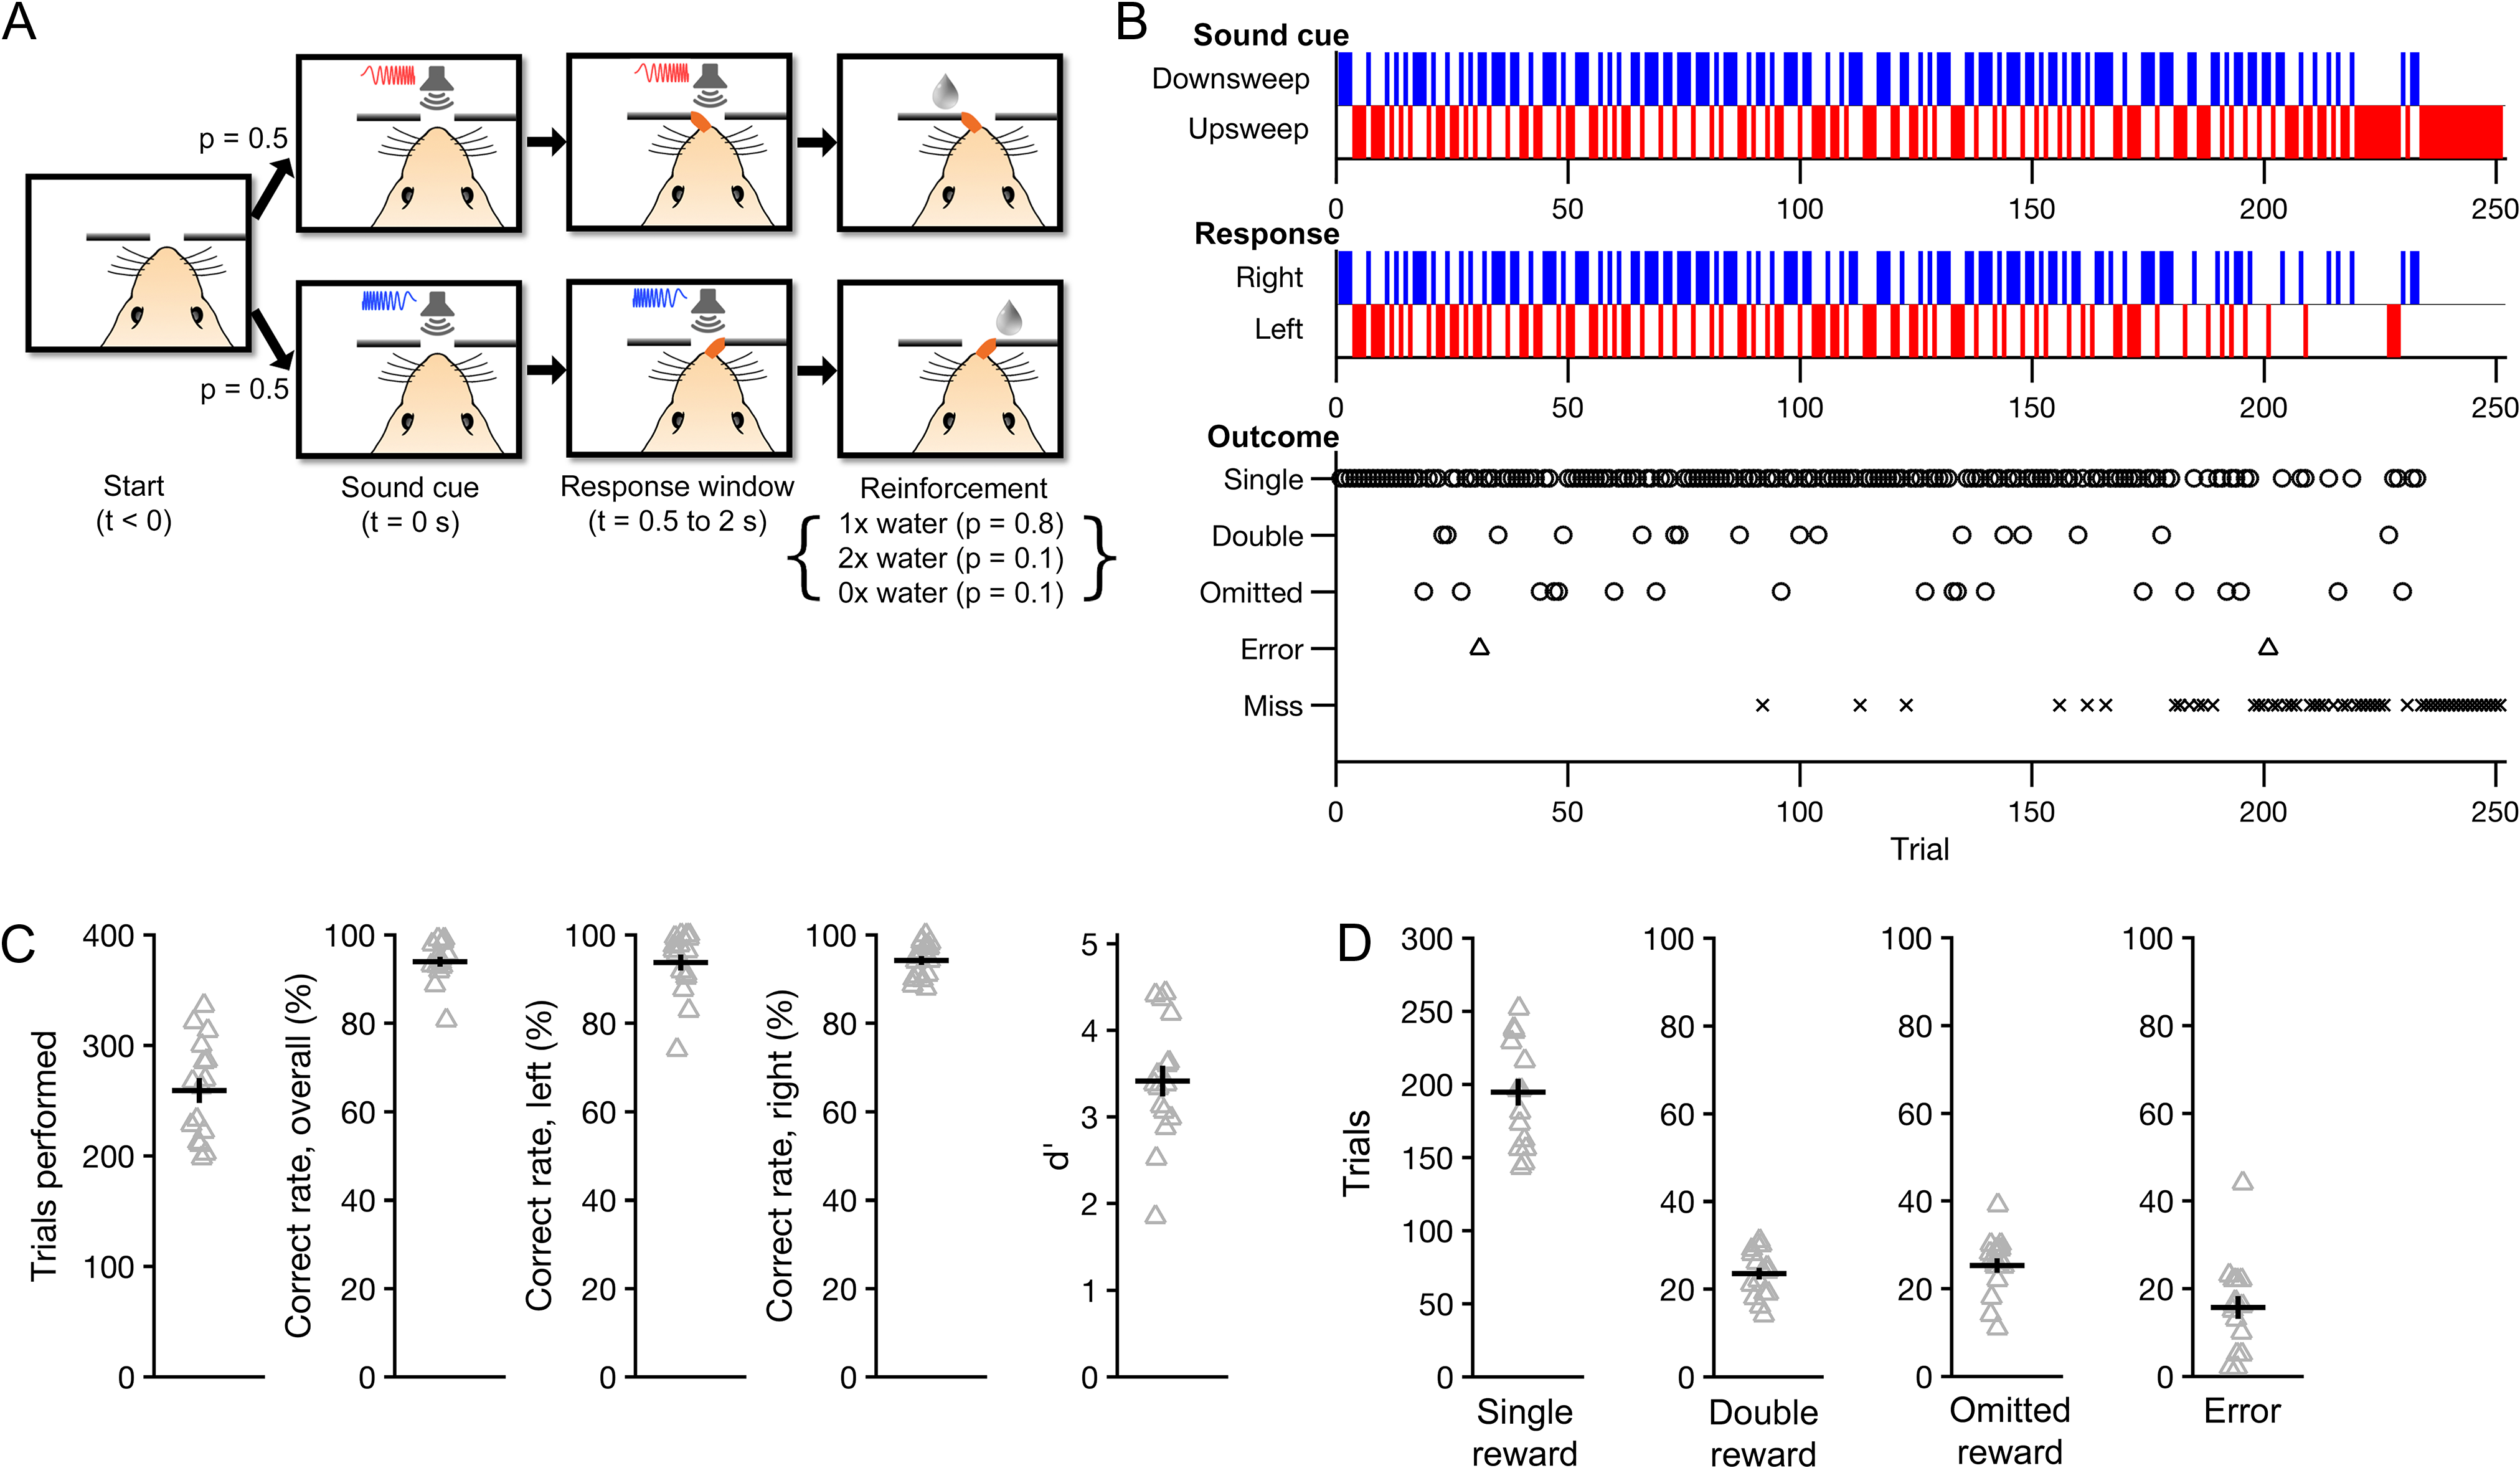
\includegraphics[width=\textwidth]{Figures/Chapter2/CC_fig1} 
\end{center}

\caption[Two-choice auditory discrimination task with probabilistic outcomes]
{Two-choice auditory discrimination task with probabilistic outcomes. On each trial, mice were required to lick the target spout (left or right) indicated by a sound cue (upsweep or downsweep, respectively). Correct responses were rewarded probabilistically with one of three water amounts. (A) Flow diagram of the trial structure on correct trials. Each trial began with one of the two sound cues. The first lick to the target spout within 0.5–2 s following cue onset (Response window) immediately triggered one of three outcomes (Reinforcement): single reward ($1\times$), double reward ($2\times$) or omitted reward ($0\times$), with probabilities 80, 10 and 10\%, respectively. The next trial would begin 7 s after cue offset. (B) Behavioral performance from an example session (Experiment 1 in Table \ref{tab:CC_table1}). Occurrences of each sound cue (top), choice (middle) and outcome (bottom) are displayed in raster form according to trial number. Errors occurred when the non-target spout was chosen for the first lick within the response window. Misses were defined by the failure to respond within the response window. (C) Summary of behavioral performance. Gray triangles, individual sessions. Black cross-hairs, $\mathit{mean}\pm\mathit{SEM}$. (D) Number of occurrences of each outcome per session. For all figures, $N = 16$ sessions from 10 mice unless otherwise noted.}

\label{fig:CC_fig1}
\end{figure}


The use of probabilistic outcomes allowed us to systematically investigate neural and behavioral effects of reward during sensorimotor decision making. In particular, the inclusion of omitted-reward trials permitted the effects of reward absence to be explicitly characterized during correct trials, thus eliminating differences in decision accuracy as a potential confound. Additionally, the influence of reward size (single reward vs. double reward) could be compared to that of its categorical presence or absence (single reward or double reward vs. omitted reward).

We obtained 16 imaging sessions from 10 mice while they performed this task (range: 1--3 sessions per mouse; Table \ref{tab:CC_table1}). Figure \ref{fig:CC_fig1} shows the behavioral performance from one such session. Subjects made $259 \pm 11$ choices per session, with an overall correct rate of $94 \pm 1\%$ ($\mathit{mean}\pm\mathit{SEM}$; Fig. \ref{fig:CC_fig1}C) and a sensitivity index ($d'$) of $3.4 \pm 0.2$. Within each session, they encountered an average of $195 \pm 9$ single-reward trials, $24 \pm 1$ double-reward trials and $25 \pm 2$ omitted-reward trials, and made $16 \pm 3$ errors. Correct rates were similar for upsweep ($94 \pm 2\%$) and downsweep ($94 \pm 1\%$) trials. Thus, subjects maintained a high level of accuracy following the introduction of variable outcomes.

\nnsub{Outcome-Dependent Behavioral Adjustments}
Subjects were well-trained in auditory discrimination before probabilistic outcomes were introduced, and the optimal stimulus–response relationships remained the same. Therefore, behavioral adjustments based on the new distribution of outcomes would not increase the overall amount of reward obtained. This raises an important question: were subjects aware of the different outcomes? 

Two lines of evidence indicate that they were. First, the number of licks to the target spout during the period following reward delivery increased in a graded manner with the volume of water reward given (Fig. \ref{fig:CC_fig2}A). On average, $13.9 \pm 0.8$ licks were registered at the target spout in single-reward trials ($\mathit{mean}\pm\mathit{SEM}$, N = 16 sessions). Relative to single-reward trials, the mean number of licks per trial rose by $21 \pm 4\%$ in double-reward trials (vs. single-reward trials: $p = 0.001$, Wilcoxon signed-rank test, $N = 16$ sessions) and decreased by $48 \pm 3\%$ in omitted-reward trials (vs. single-reward trials: $p = 4 \times 10^{-4}$, Wilcoxon signed-rank test, $N = 16$ sessions). Because the different outcome types were interleaved randomly across correct trials, these results indicate that the mice could detect changes in reward volume and adjusted their consummatory licking accordingly.

\begin{figure}[htbp]

\begin{center}
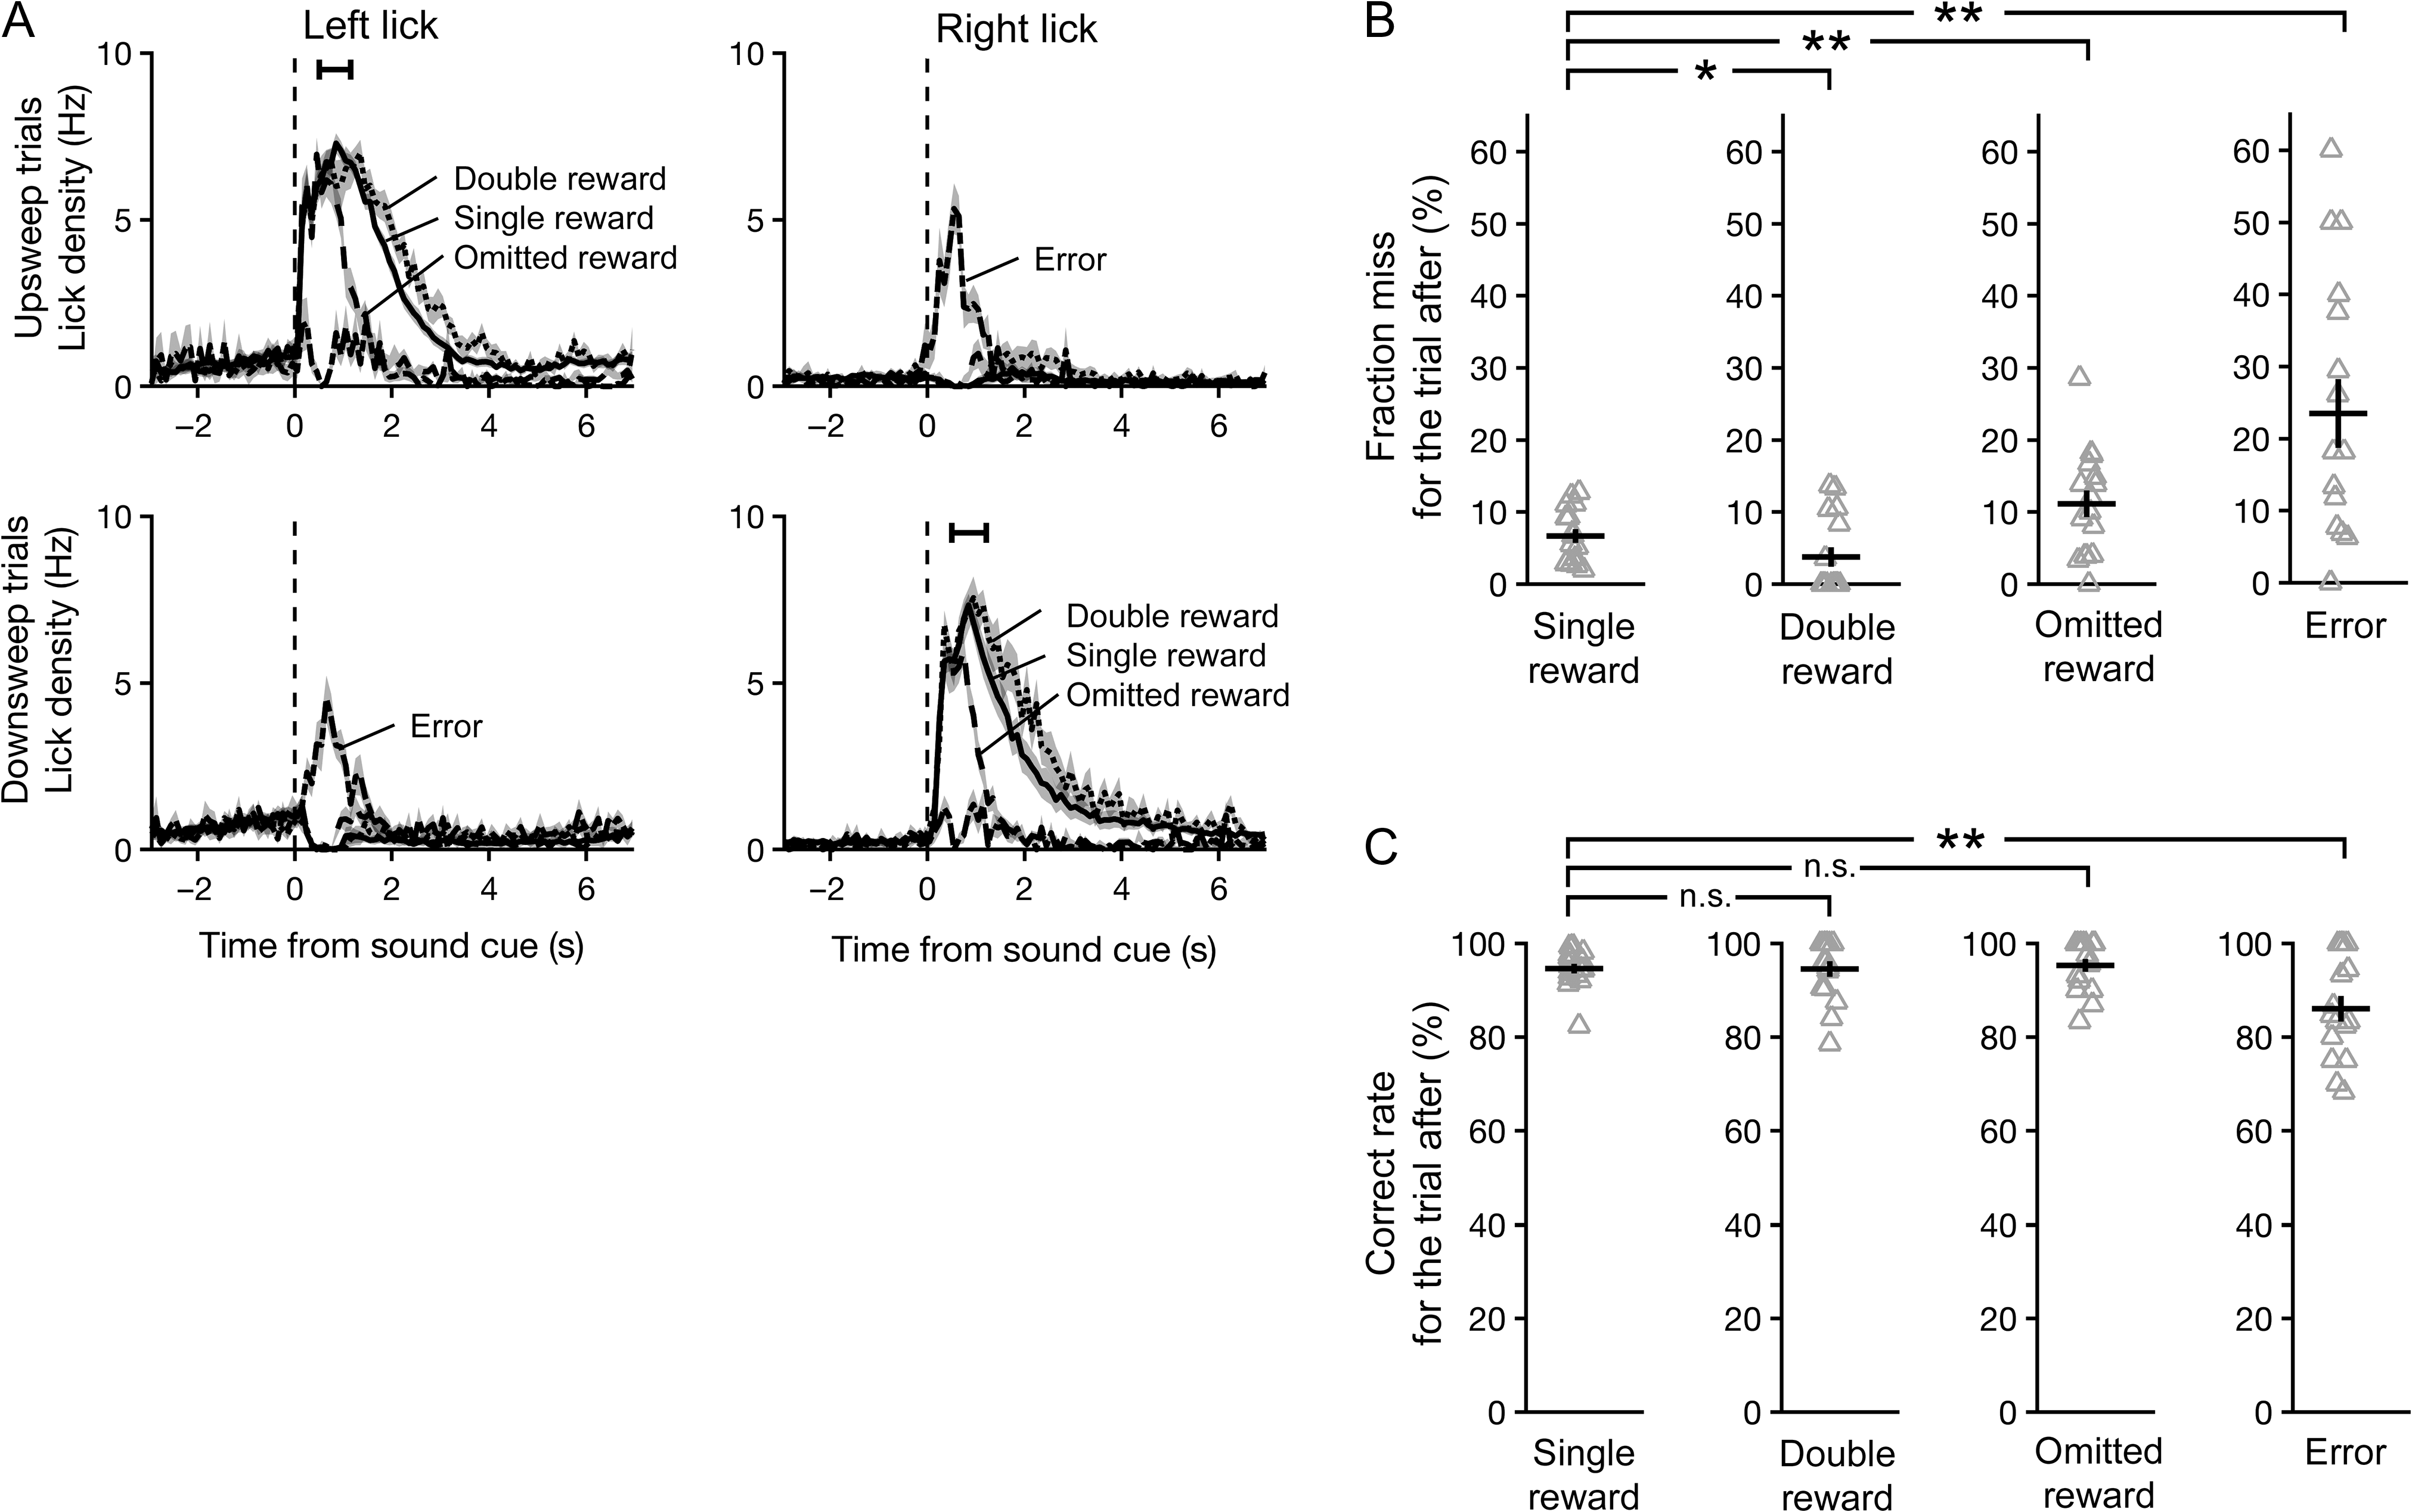
\includegraphics[width=\textwidth]{Figures/Chapter2/CC_fig2} 
\end{center}

\caption[Outcome-dependent behavioral adjustments]
{Subjects adjusted their behavior based on trial outcome. (A) Mean lick density across sessions as a function of time for the left and right spouts, averaged separately from trials in which the sound cue was an upsweep (top row) or downsweep (bottom row), and outcome was single reward (solid), double reward (dotted) or omitted reward (dashed). Black error bar, 95\% confidence interval for time of outcome. (B) Fraction of trials missed immediately following each outcome. Gray triangles, individual sessions. Black crosshairs, $\mathit{mean}\pm\mathit{SEM}$. Wilcoxon signed-rank test: *$p < 0.05$, **$p < 0.005$, n.s., not significant. (C) Fraction of trials with a correct response immediately following each outcome.}

\label{fig:CC_fig2}
\end{figure}

Second, behavioral performance varied as a function of the prior trial’s outcome. The most notable effect was on the number of misses (Fig. \ref{fig:CC_fig2}B). The likelihood of a miss was $7 \pm 1\%$ for trials following a single reward ($\mathit{mean}\pm\mathit{SEM}$, $N = 16$ sessions). It was significantly lower at $4 \pm 1\%$ for trials following a double reward ($p = 0.04$, Wilcoxon signed-rank test, $N = 16$ sessions) but significantly higher at $11 \pm 2\%$ if reward was omitted in the previous trial (vs. single-reward trials: $p = 0.005$, Wilcoxon signed-rank test, $N = 16$ sessions). However, when subjects did respond, the correct rate was consistently high at $95 \pm 1$, $95 \pm 2$ and $95 \pm 1\%$ for trials following a single, double and omitted rewards, respectively (Fig. \ref{fig:CC_fig2}C; $\mathit{mean}\pm\mathit{SEM}$, $N = 16$ sessions). Taken together, the observed adjustments in licking and the effect on miss rate in the subsequent trial provide clear evidence that the mice monitored trial outcomes. Notably, the magnitude of reinforcement affected subjects’ willingness to respond, but did not influence the accuracy of decisions.

\nnsub{Persistent Decline in Performance Following Errors}
Errors were uncommon in these experiments. However, inference to the causes of residual inaccuracy could help to illuminate internal processes underlying decision making. Our task design permitted us to examine and rule out two potential sources of error. First, errors could have resulted mainly from stochastic fluctuations in perceptual performance. In this case, the likelihood of a correct response should not depend significantly on recent performance history. Thus, similar levels of performance would be expected in trials following errors and correct responses. However, relative to correct responses, errors were associated with deficits in both decision accuracy and willingness to respond in the subsequent trial. Correct rate dropped to $86 \pm 3\%$ in trials following an error (Fig. \ref{fig:CC_fig2}C; vs. single-reward trials: $p = 0.01$; vs. omitted-reward trials: $p = 0.01$; Wilcoxon signed-rank test, $N = 16$ sessions), and miss rate increased to $23 \pm 5\%$ (Fig. \ref{fig:CC_fig2}B; vs. single-reward trials: $p = 0.004$; vs. omitted-reward trials: $p = 0.04$, Wilcoxon signed-rank test, $N = 16$ sessions). We also asked whether the likelihood of an error could be explained by outcome-dependent processes, such as exploration following the absence of an expected reward. This hypothesis is not supported by the observation that error rates following correct trials were similar regardless of the prior trial’s outcome (Fig. \ref{fig:CC_fig2}C). Collectively, our results suggest that the drop in task performance associated with errors tends to persist and cannot be solely accounted for by the trial outcome.

\nnsub{Single-Unit Activity Related to Choices and Outcomes}
To characterize neural activity in M2 while mice engaged in the task, we simultaneously imaged the brain at cellular resolution using a two-photon microscope \citep{denk1990two} (Fig. \ref{fig:CC_fig3}A). An adeno-associated virus encoding GCaMP6s (AAV1.Syn.GCaMP6s.WPRE.SV40) was injected into layer 2/3 of M2, and a chronic glass window was implanted for optical imaging (Fig. \ref{fig:CC_fig3}B). GCaMP6s is a genetically encoded calcium indicator that exhibits an approximately 25\% rise in fluorescence intensity per action potential in cortical pyramidal neurons \citep{chen2013ultrasensitive}. In 16 imaging sessions, we recorded fluorescence transients from an average of $48 \pm 3$ neurons in layer 2/3 of M2 ($\mathit{mean}\pm\mathit{SEM}$, range: 33–77 cells; Fig. \ref{fig:CC_fig3}C). All imaging was done in the right hemisphere; therefore, left and right licks were always contralateral and ipsilateral to the imaged neurons, respectively.

\begin{figure}[htbp]

\begin{center}
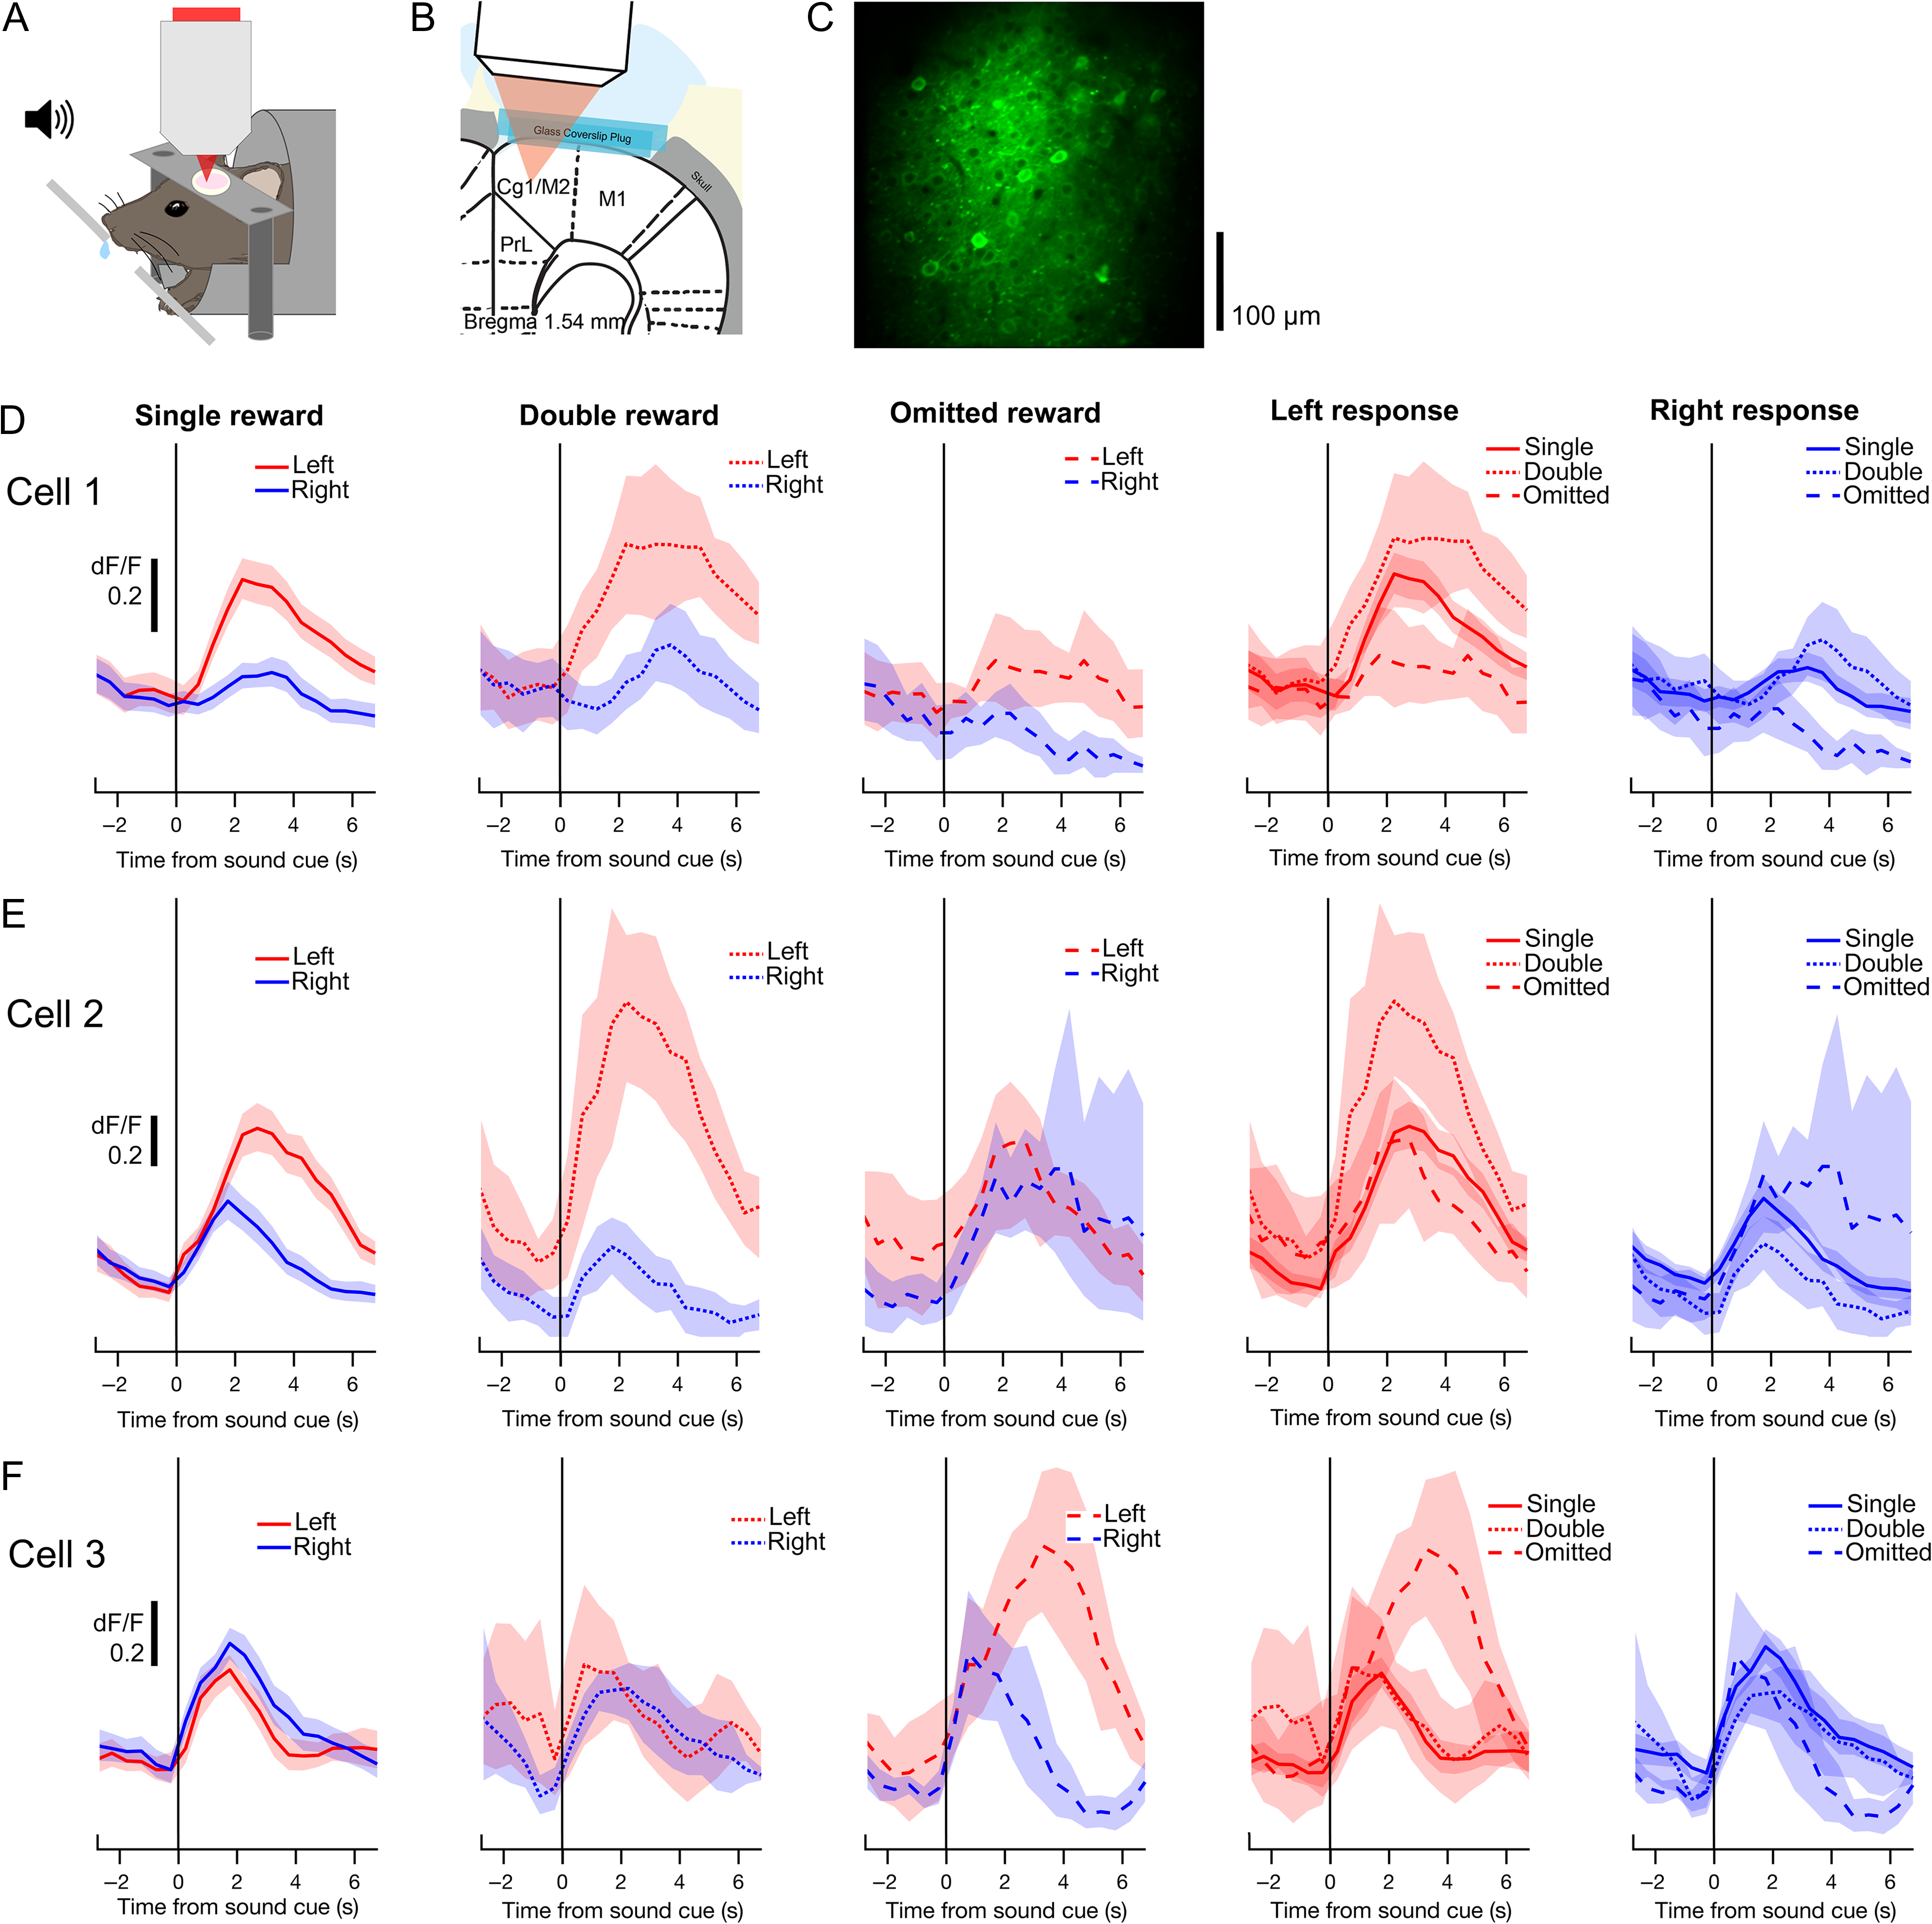
\includegraphics[width=\textwidth]{Figures/Chapter2/CC_fig3} 
\end{center}

\caption[Two-photon Ca\textsuperscript{2+} imaging of choice- and outcome-related signals]
{Two-photon calcium imaging of choice- and outcome-related signals in secondary motor cortex (M2). (A) Schematic representation of experimental setup for behavior with simultaneous two-photon imaging. (B) Schematic representation of preparation for in vivo two-photon imaging of M2. PrL, prelimbic cortex; Cg1, cingulate area 1; M1, primary motor cortex. (C) An example field-of-view in layer 2/3 of M2 containing GCaMP6s-expressing neurons. The image is a mean projection of the full time-lapse image stack from Experiment 13 in Table 1. (D) Mean fluorescence traces from an example cell, aligned to the sound cue and averaged across different subsets of trials. In the leftmost three panels, traces from left (red) and right (blue) trials are overlaid for each trial outcome. The rightmost two panels display the same data, with traces from single- (solid), double- (dotted) and omitted-reward trials (dashed) overlaid for each chosen action. Shading, 90\% confidence interval. (E–F) Same as D for two additional cells.}

\label{fig:CC_fig3}
\end{figure}

Many M2 neurons exhibited changes in fluorescence following the sound cue, indicating task-driven neural activity. Figure \ref{fig:CC_fig3}D shows a neuron with preferential activity on trials in which the left spout was chosen. The activity of the same neuron was also monotonically modulated by reward size: activity was highest for double rewards, moderate for single rewards and lowest for omitted rewards. The influence of choice and outcome on this neuron was approximately additive. However, other neurons had more complex responses. Some neurons showed a choice preference on single- and double-reward trials that was not observed on omitted-reward trials, suggesting a choice–outcome interaction (Fig. \ref{fig:CC_fig3}E). Other neurons only exhibited significant choice preference during omitted-reward trials (Fig. \ref{fig:CC_fig3}F). These results highlight the diversity of choice- and outcome-related signals in M2 at the level of individual neurons.

\nnsub{Persistence of Choice- and Outcome-Related Signals}
To more systematically characterize choice- and outcome-related signals in M2 neurons, we used multiple linear regression analysis. For each cell, we fit a linear equation (see Materials and Methods) to estimate the dependence of its fluorescence intensity on the following predictors: choice, outcome, and the interaction of choice and outcome; for the current trial, last trial, and the trial before last (Fig. \ref{fig:CC_fig4}A). The analysis revealed choice-dependent activity in a substantial fraction of M2 neurons (210/771 cells, 27\%; $p < 0.01$ for the corresponding regression coefficient in at least five consecutive time-bins, binomial test; Fig. \ref{fig:CC_fig4}B). Dependence on outcome (42 cells, 5\%; Fig. \ref{fig:CC_fig4}C) or a choice–outcome interaction (25 cells, 3\%; Fig. \ref{fig:CC_fig4}D) was evident in comparatively fewer cells. Notably, significant fractions of M2 neurons continued to show choice- and outcome-dependent signals well into the next trial, persisting even after the next choice was made (black bars denoting $p < 0.01$, binomial test, middle panel, Fig. \ref{fig:CC_fig4}B–D).

\begin{FPfigure}

\begin{center}
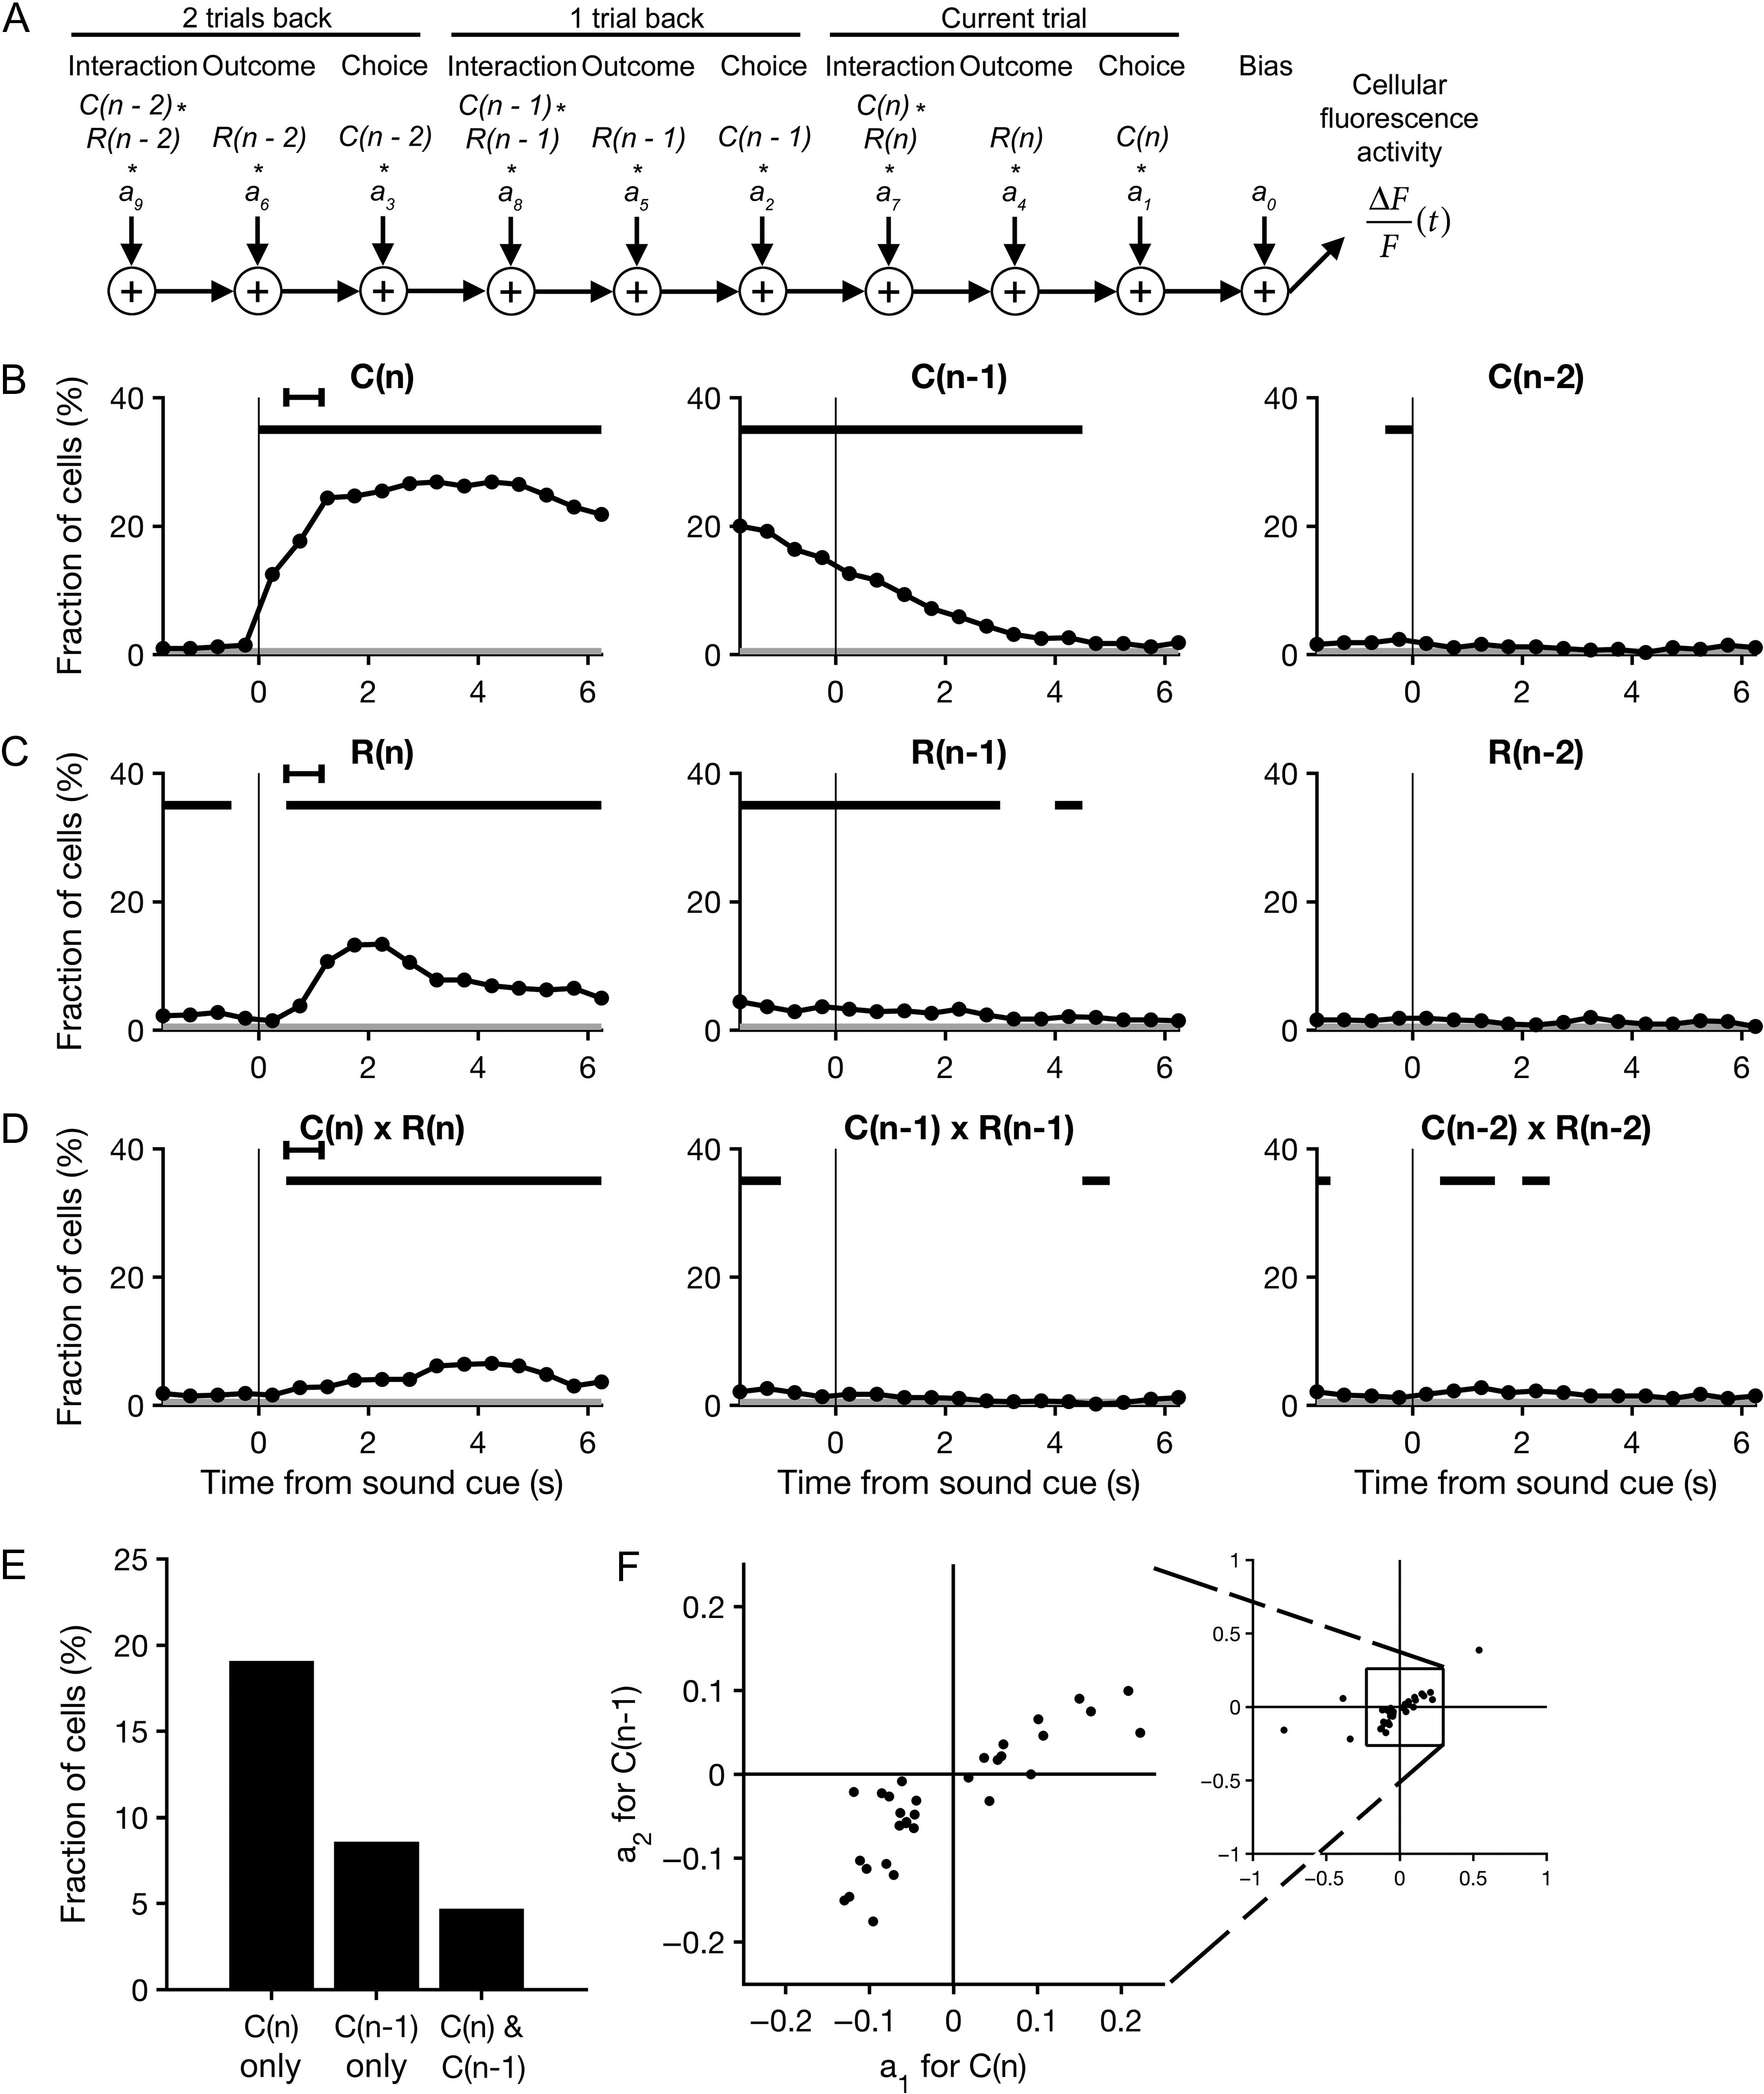
\includegraphics[width=\textwidth]{Figures/Chapter2/CC_fig4} 
\small{Figure \ref{fig:CC_fig4} Sustained representations of choices and their outcomes in M2.}
\end{center}

\caption[Sustained representations of choices and their outcomes]
{Sustained representations of choices and their outcomes in M2. (A) A schematic representation of the multiple linear regression model that was fit to the fluorescence of each neuron in each 500 ms time bin. (B) The proportion of cells with significant choice-dependent activity as quantified by the regression model, plotted as a function of time. The regression model accounted for the influence of choices made on the current trial (left), the last trial (middle) and the trial before last (right), as well as the additional predictors shown in C–D. Significance of each predictor was tested at $\alpha = 0.01$. Black bars, bins in which the proportion of cells with significant regression coefficients was above chance level ($p < 0.01$, binomial test). Gray shading, the significance threshold for the binomial test. Black error bar, 95\% CI for time of outcome. $N = 771$ cells from 16 sessions from 10 mice. (C) Same as B for trial outcome. (D) Same as B for the interaction of choice and outcome. (E) The proportion of neurons with a significant regression coefficient for the choice made in the current trial only, in the prior trial only, and in both the current and prior trials. (F) Scatter plot of the neurons with significant regression coefficients for both the current and prior choice. The coefficient for the current choice, $a_1$, is plotted against the coefficient for the prior choice, $a_2$. Right inset, the same plot expanded to show the five data points outside the range of the main axis.}
\clearpage
\label{fig:CC_fig4}
\end{FPfigure}

The observation that M2 neurons can represent chosen actions across more than one trial led us to ask whether current and prior choices are represented at the single-unit level by the same or different populations. To address this question, we quantified the number of neurons with a significant regression coefficient only for the current choice ($p < 0.01$ for $a_1$, the regression coefficient for the current choice estimated 2 s after cue onset, and $p \geq 0.01$ for $a_2$, the regression coefficient for the prior choice estimated at the time of cue onset), only for the prior choice ($p \geq 0.01$ for $a_1$ and $p < 0.01$ for $a_2$) and for both the current and prior choices ($p < 0.01$ for both $a_1$ and $a_2$). We found that most choice-dependent M2 neurons were sensitive exclusively to the current (147/771 cells, 19\%) or prior (66/771 cells, 9\%) choice (Fig. \ref{fig:CC_fig4}E). Within the small proportion of neurons sensitive to both current and prior choices (36/771 cells, 5\%), the corresponding regression coefficients were correlated and generally did not change signs (Fig. \ref{fig:CC_fig4}F). Therefore, the choice preferences of these cells were maintained across time-points in consecutive trials. Taken together, these results indicate that very few of the choice-selective neurons in M2 represent both the current and prior choice during the period immediately following cue onset.

%***Resume Initial Formatting Here*** 
\nnsub{Effect of Outcome on Choice Selectivity of Single Neurons}
To further characterize choice representations in M2, we focused on the 226 ‘choice-selective’ neurons whose activity was found in the multiple linear regression analysis to be significantly modulated by choice, or the interaction of choice and outcome, or both. For each of these neurons, fluorescence traces were first averaged across subsets of trials according to whether the contralateral (left) or ipsilateral (right) spout was chosen (trial-averaged traces for each cell during single reward, left trials are shown in Fig. \ref{fig:CC_fig5}A). A time-varying choice selectivity index was then calculated as the normalized difference between the two mean traces. During the period following cue onset in single-reward trials, the majority of choice-selective neurons preferred the contralateral choice (134/226, 59\%; Fig. \ref{fig:CC_fig5}B). Similar to the degree of temporal variation observed across neurons in their trial-averaged activity traces, peak choice selectivity was also temporally distributed across neurons relative to the sound cue (Fig. \ref{fig:CC_fig5}A,B).

\begin{figure}[htbp]

\begin{center}
\includegraphics[width=\textwidth]{Figures/Chapter2/CC_fig5} 
\end{center}

\caption[Choice representations were modified by trial outcome]
{Choice representations in M2 are modified by trial outcome. (A) Heat map of trial-averaged fluorescence as a function of time for all choice-selective neurons during single-reward, left trials. Cells are sorted by the center-of-mass of their trial-averaged fluorescence traces. $n = 226$ cells with significant encoding of choice or an interaction of choice and outcome as determined by multiple linear regression (see Methods). (B) Heat map of choice selectivity for the neurons in A as a function of time during single-reward trials. Choice selectivity was calculated as the normalized difference between mean fluorescence traces from left and right trials. Red and blue shadings indicate preference for left and right choices, respectively. Cells are sorted first by mean choice preference and then by the center-of-mass of their choice selectivity traces. (C) Scatter plot of the neurons in A, plotting the choice selectivity of each cell in omitted-reward trials against double-reward trials. $R$, Pearson correlation coefficient. (D) Empirical cumulative distribution of choice selectivity magnitudes for double-reward (solid) and omitted-reward (dotted) trials.}

\label{fig:CC_fig5}
\end{figure}

Unexpected outcomes signify inaccuracies within a subject’s internal representation of the environment, including the values assigned to specific actions. Such information can be crucial to instrumental behavior. Thus, we asked whether choice representations in M2 were modified when low-probability outcomes occurred. Specifically, we examined double- and omitted-reward trials, which occurred a similar number of times per session. The choice selectivity of individual neurons clearly varied by trial type, as evidenced by the degree of scatter from the unity line in Figure \ref{fig:CC_fig5}C. Nevertheless, across the choice-selective neurons, the choice selectivity values for double- and omitted-reward trials were significantly correlated (Pearson's $R = 0.31$, $p = 5 \times 10^{-6}$, $N = 226$ cells). Notably, choice selectivity magnitudes were reduced on omitted reward as compared to double-reward trials ($p = 5 \times 10^{-5}$, Wilcoxon signed-rank test; Fig. \ref{fig:CC_fig5}D). Extending this analysis to include all imaged neurons yielded similarly correlated choice selectivity values ($R = 0.20$, $p = 2 \times 10^{-8}$, $N = 771$ cells) and a similar reduction in choice selectivity magnitudes for omitted reward relative to double-reward trials ($p = 0.002$, Wilcoxon signed-rank test). These results indicate that trial outcomes can substantially influence choice representations in M2. In particular, the absence of an expected reward in omitted-reward trials was associated with weaker representations of chosen actions at the level of single neurons.

\nnsub{Reward Omission Weakened Population-Level Choice Representations}
Frontal cortical neurons often exhibit complex patterns of selectivity for task variables, and mounting evidence suggests that the associated neural representations may be best understood by focusing on the activity of large populations of neurons, rather than single units. Therefore, relative to the single-unit analyses presented above, the measure of accuracy at decoding choices from ensemble activity could provide a more reliable estimate of the choice information available to downstream brain areas.

To test the effect of trial outcomes on population-level choice representations in M2, we trained linear classifiers on the ensemble activity recorded during single-reward trials and then compared their accuracy for decoding choices across trials with different outcomes (see Materials and Methods). Baseline decoding accuracy was estimated with a Monte Carlo cross-validation procedure, using ensemble activity patterns from single-reward trials as training and testing sets. For each of 30 iterations, a classifier was constructed from a random sample of 80\% of these trials and then tested on the remaining fraction. Decoding accuracy for the other outcome types was estimated by testing the same classifiers on the ensemble activity associated with the full set of double-reward, omitted-reward and error trials.

The choices made in correct trials could be decoded from the population activity with above chance-level accuracy at every time-point in the current trial following the animal’s response (Fig. \ref{fig:CC_fig6}A–C, left; black bar denotes $p < 0.05$, Wilcoxon signed-rank test, vs. shuffle). An ensemble representation of the chosen action could also be detected for at least 1 s into the subsequent trial (Fig. \ref{fig:CC_fig6}A–C, right). For example, in single-reward trials, a maximal decoding accuracy of $78 \pm 2\%$ was reached at 1.75 s after cue onset ($\mathit{mean}\pm\mathit{SEM}$, $N = 16$ sessions; Fig. \ref{fig:CC_fig6}A, left). At the time of the next cue onset, accuracy remained above chance, at $63 \pm 2\%$ ($\mathit{mean}\pm\mathit{SEM}$, $N = 16$ sessions; Fig. \ref{fig:CC_fig6}A, right). By contrast, in error trials, the decoding accuracy increased gradually from the time of cue onset (Spearman's $\rho = 0.87$, $p < 10^{-4}$) and only rose to significance late in the trial (Fig. \ref{fig:CC_fig6}D, left). It reached a maximum of $66 \pm 4\%$ at the time of the next sound cue ($\mathit{mean}\pm\mathit{SEM}$, $N = 16$ sessions; Fig. \ref{fig:CC_fig6}D, right).

\begin{FPfigure}

\begin{center}
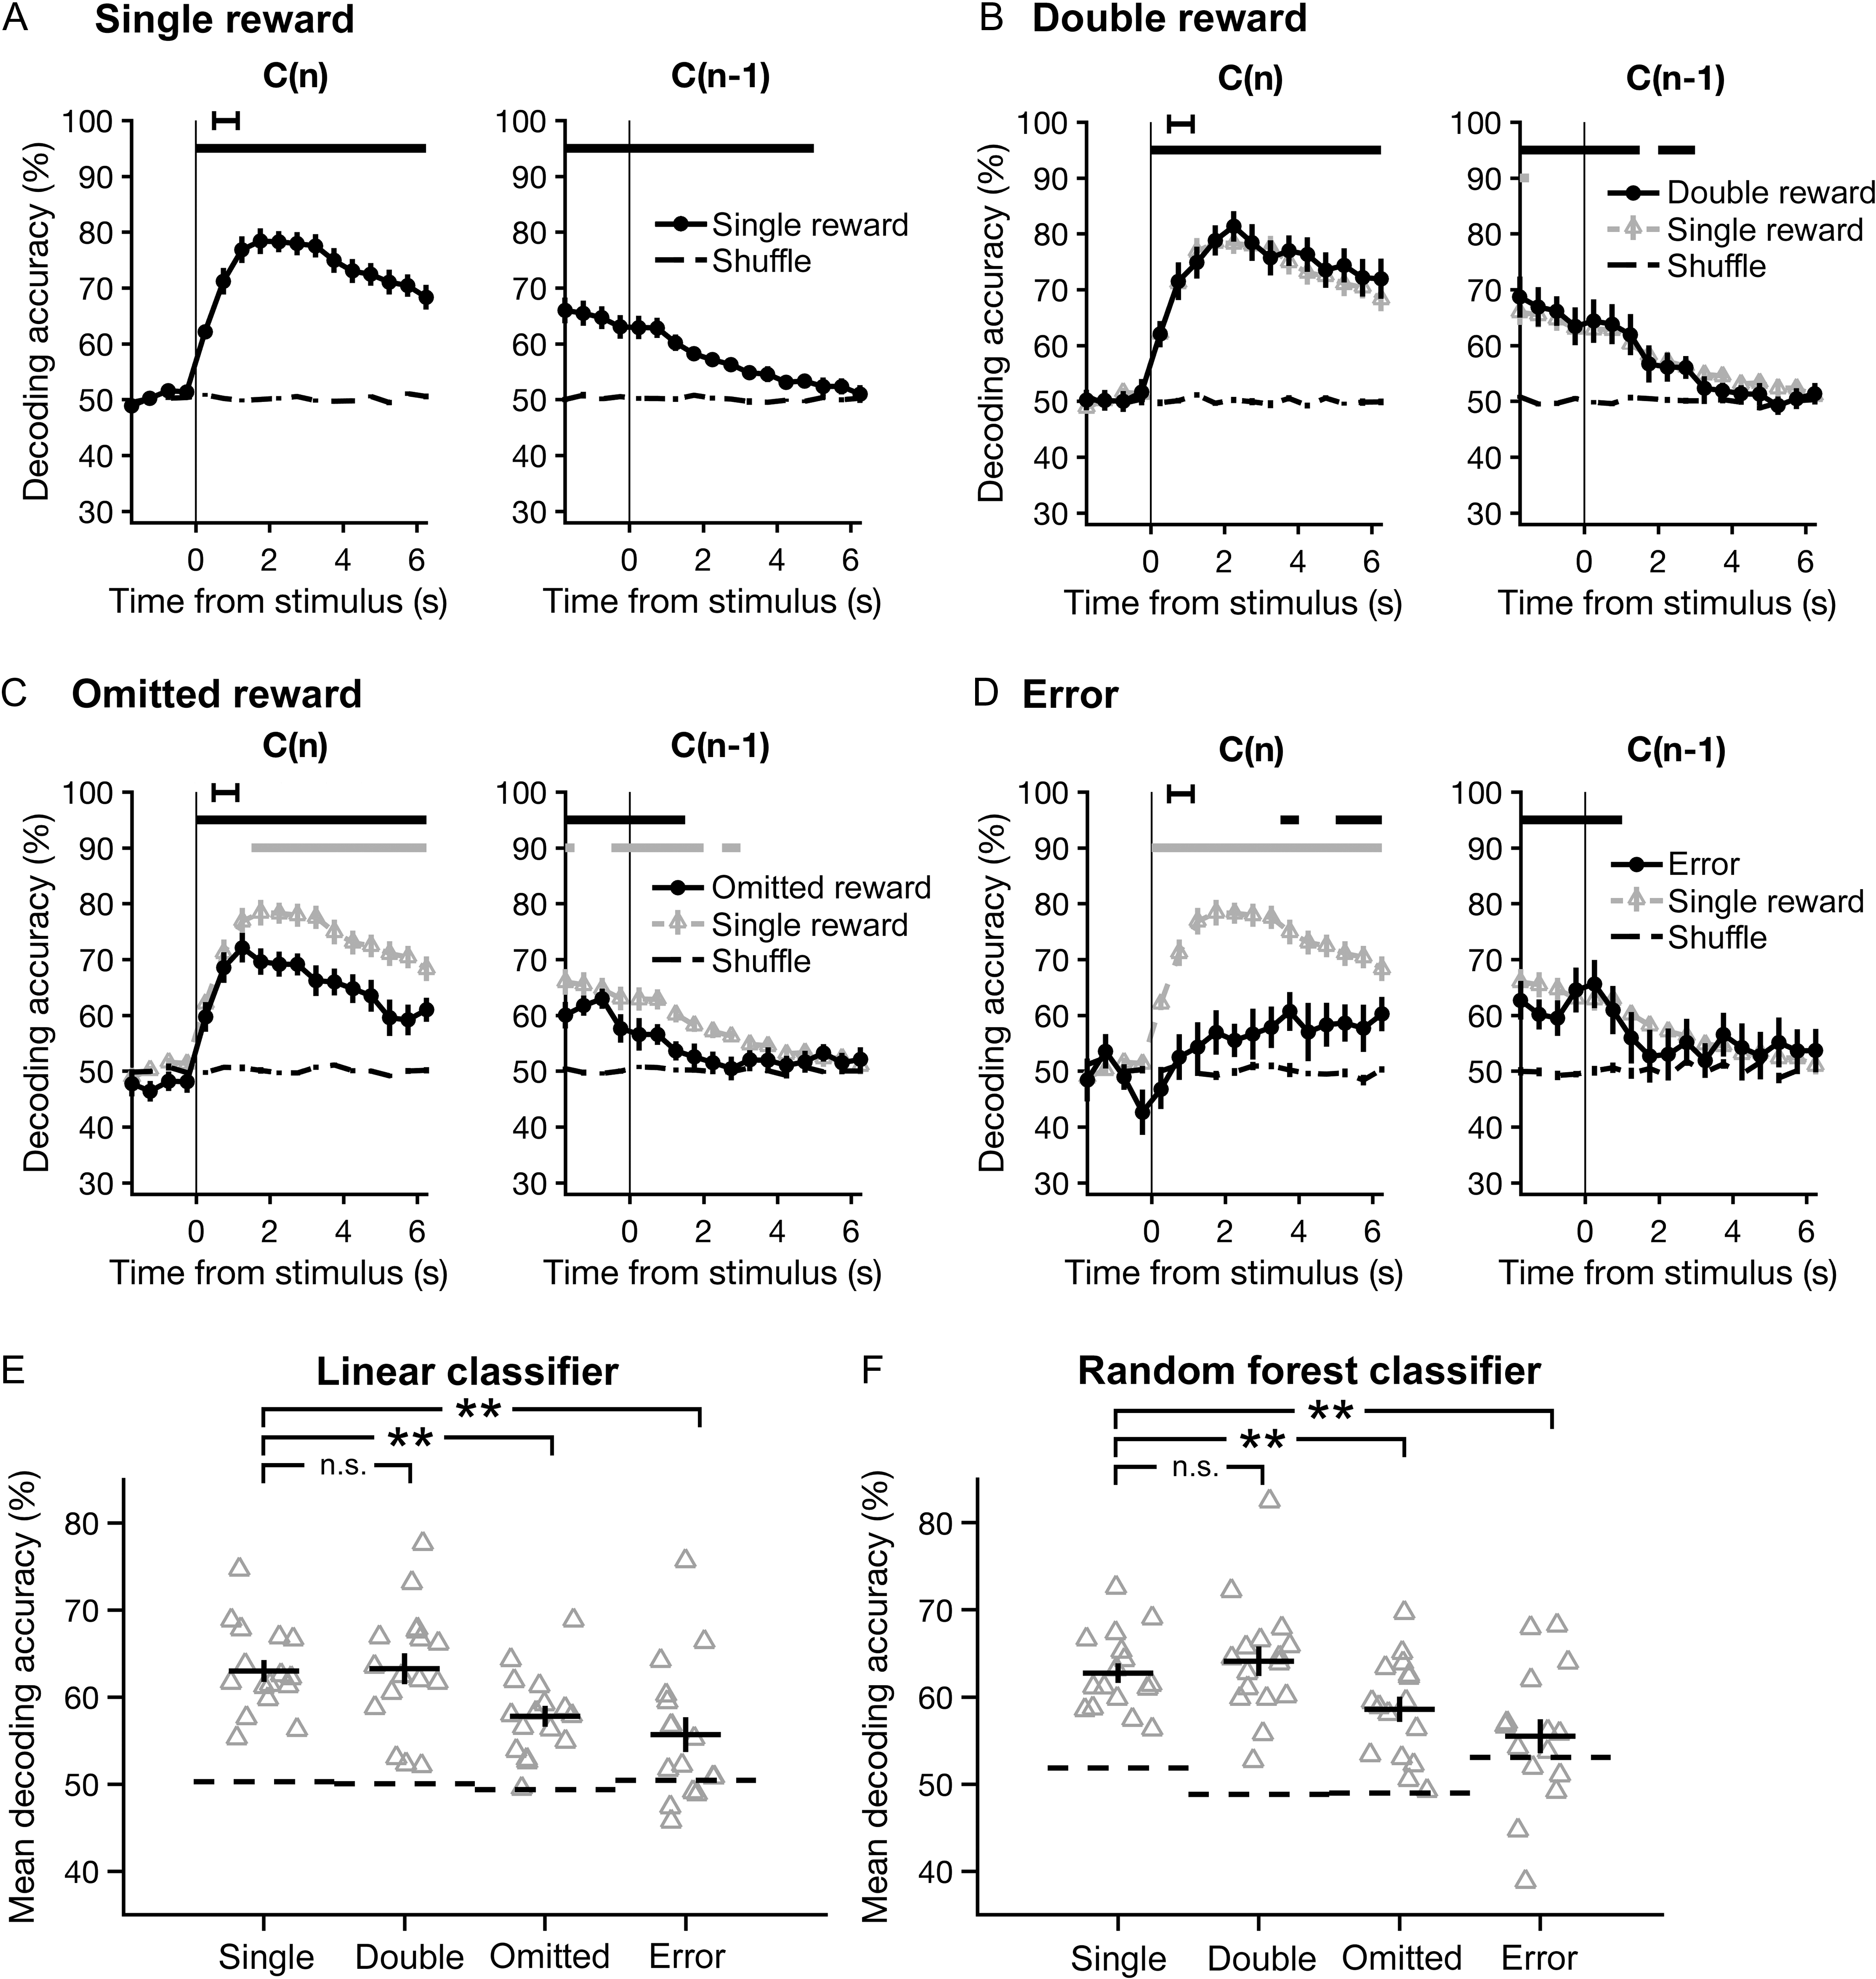
\includegraphics[width=\textwidth]{Figures/Chapter2/CC_fig6} 
\small{Figure \ref{fig:CC_fig6}: Decoding accuracy diminished during omitted-reward and error trials. }
\end{center}

\caption[Decoding accuracy diminished during omitted-reward and error trials]
{The accuracy of decoding chosen actions from the neural ensemble activity was diminished during omitted-reward and error trials. Choices were decoded using classifiers based on linear discriminant analysis, and accuracy was estimated with Monte Carlo cross-validation (repeated random subsampling). (A) The accuracy of decoding choices made on single-reward trials (left), or trials in which the previous outcome was single reward (right), plotted as a function of time. Data are presented as $\mathit{mean}\pm\mathit{SEM}$. Chance-level accuracy (black dashed line) was determined by testing classifiers constructed using shuffled choices. Black horizontal bars, bins significantly different from chance ($p < 0.05$, Wilcoxon signed-rank test). Black error bar, 95\% confidence interval for time of outcome. (B-D) Same as A for double-reward, omitted-reward, and error trials. Results from single-reward trials are overlaid for visual comparison (gray triangles). Lower gray bars, bins with a significant difference in decoding accuracy relative to single-reward trials. (E) Mean decoding accuracy across all time-points shown in A–D for each trial outcome. Gray triangles, individual sessions. Black crosshairs, $\mathit{mean}\pm\mathit{SEM}$. Wilcoxon signed-rank test: **$p < 0.01$; n.s., not significant. (F) Same as E using random forest classifiers.}
% \clearpage %\placefloats places without an automatic new page
\label{fig:CC_fig6}
\end{FPfigure}

For explicit comparisons of decoding accuracy across outcome conditions, we computed the mean accuracy over all time-points in the current and subsequent trial (Fig. \ref{fig:CC_fig6}E). Relative to single-reward trials, mean decoding accuracy dropped significantly in omitted-reward ($p = 0.004$, Wilcoxon signed-rank test, $N = 16$ sessions) and error trials ($p = 0.002$, Wilcoxon signed-rank test, $N = 16$ sessions), with no detectable difference in double-reward trials ($p = 0.8$, Wilcoxon signed-rank test, $N = 16$ sessions).

It seems unlikely that the choice information present in M2 ensemble activity would be read out by the brain in exactly the same manner as a linear classifier. Therefore, we sought an alternative approach to determine whether the results would generalize to other methods of decoding. Specifically, we turned to random forest classification, a bootstrap aggregation method based on decision trees. Random forest classifiers operate on a fundamentally different principle than linear classifiers (see Materials and Methods), but overall, they yielded very similar results. In particular, comparisons of mean decoding accuracy again revealed marked differences between single-reward trials and omitted-reward or error trials ($p =$ 0.006 and 0.003, respectively, Wilcoxon signed-rank test, $N = 16$ sessions), but no difference between single- and double-reward trials ($p = 0.2$, Wilcoxon signed-rank test, $N = 16$ sessions; Fig. \ref{fig:CC_fig6}F). Thus, the results of two distinct classification approaches support the same conclusion: that choice information was encoded with higher fidelity during trials in which choices were rewarded. More specifically, increases in reward magnitude (ie double reward) had little impact on decoding accuracy, whereas reward absence in omitted-reward and error trials significantly diminished the accuracy with which chosen actions could be decoded from neural ensemble activity patterns in M2.

\nnsub{Simultaneous Recording Improved Decoding Accuracy}
Our measurements of neural activity came from two-photon calcium imaging, which enabled the simultaneous acquisition of fluorescence transients from ensembles of at least 30 neurons. This allowed us to address an important, unresolved methodological question: does simultaneous recording confer a decoding advantage, relative to recording from each cell individually and then combining the data post hoc \emph{in silico}?

As a basis for comparison, we generated ‘pseudo-ensemble’ data for each session, in which the activity traces from each neuron were shuffled across single-reward trials where the same action was chosen. Thus, the correspondence between individual neural activity traces and left or right choices was preserved. However, at the population level, the ensemble activity patterns no longer reflected simultaneously recorded activity. In particular, the shuffle should preserve co-fluctuations in neural activity related to the sound cue, choice and outcome of a given trial, while disrupting the residual correlations.

To determine the extent to which correlations in neural activity were disrupted by the shuffling procedure, we first determined the correlation between each pair of neurons across trials, using the mean cellular fluorescence over the time interval from 2 to 4 s after cue onset (Fig. \ref{fig:CC_fig7}A). As expected, pairwise correlations were reduced within the pseudo-ensembles (Fig. \ref{fig:CC_fig7}B). Across all sessions, the mean Pearson correlation coefficient decreased from $0.173 \pm 0.020$ in simultaneously recorded ensembles to $0.022 \pm 0.007$ in pseudo-ensembles ($p = 4 \times 10^{-4}$, Wilcoxon signed-rank test; Fig. \ref{fig:CC_fig7}C, left). The mean magnitude of correlation also decreased, from $0.192 \pm 0.017$ in simultaneously recorded ensembles to $0.054 \pm 0.005$ in pseudo-ensembles ($p = 4 \times 10^{-4}$, Wilcoxon signed-rank test; Fig. \ref{fig:CC_fig7}C, right).

\begin{FPfigure}

\begin{center}
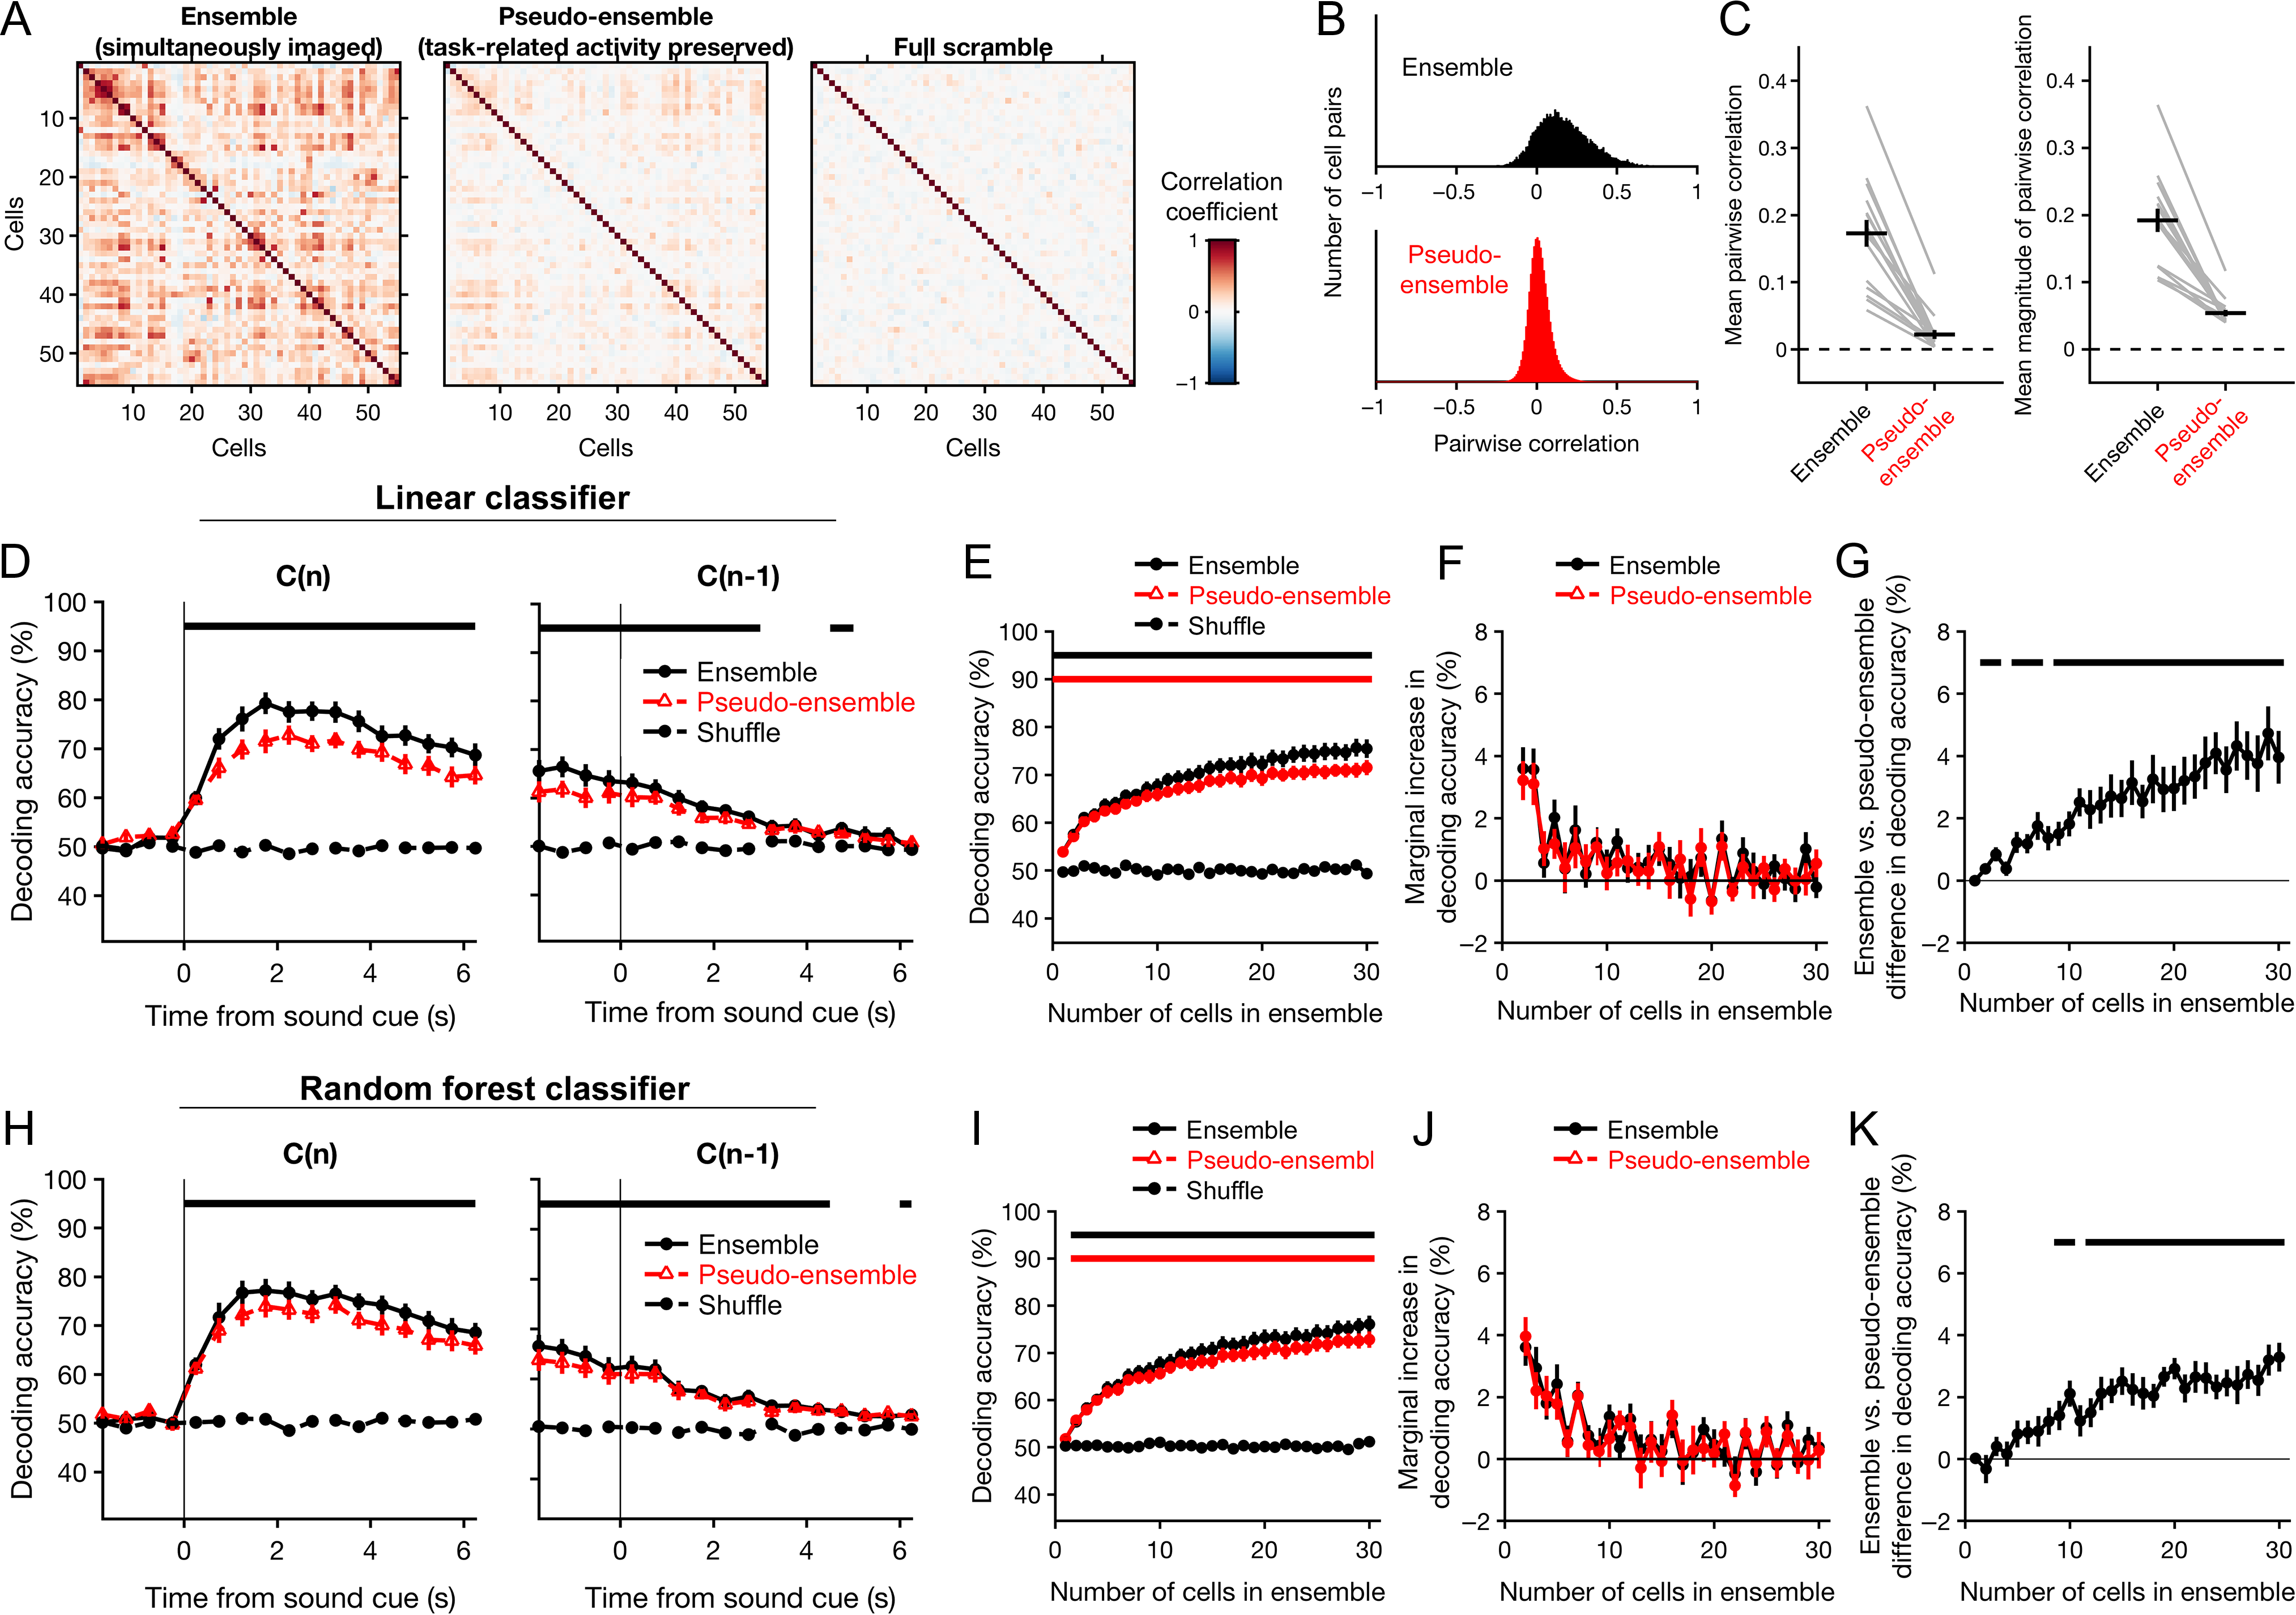
\includegraphics[width=\textwidth]{Figures/Chapter2/CC_fig7} 
\small{Figure \ref{fig:CC_fig7}: Decoding advantage of simultaneous recording increased with ensemble size.}
\end{center}

\caption[Decoding advantage of simultaneous recording increased with ensemble size]
{Simultaneous recording imparted a decoding advantage that increased as a function of ensemble size. The accuracy of decoding choices from the activity of simultaneously imaged ensembles of neurons was compared to that of pseudo-ensembles in which simultaneity was disrupted by shuffling the activity traces from each neuron across trials in which the same choice was made. Only correct trials resulting in a single reward were used for this analysis. Classification accuracy was tested using Monte Carlo cross-validation (repeated random subsampling). Chance-level accuracy was determined by testing classifiers constructed using shuffled choices. (A) Pearson correlation matrix for all cells from one example session, under three conditions: with simultaneity preserved (‘ensemble’), after shuffling across trials with the same chosen action (‘pseudo-ensemble’), and after shuffling across trials irrespective of chosen action (‘full scramble’). Correlations were estimated from cellular fluorescence averaged over the interval from 2--4 s following cue onset. (B) Histogram of the Pearson correlation coefficients estimated for all pairs of cells imaged in all experiments, using simultaneous ensembles (top) and pseudo-ensembles (bottom). (C) Mean pairwise correlation (left), and pairwise correlation magnitude (right) across all sessions. Gray lines, means from individual sessions. Black crosshairs, grand $\mathit{mean}\pm\mathit{SEM}$. (D) Performance of decoders based on linear discriminant analysis, plotted as a function of time for single-reward trials (left), or trials in which the previous outcome was a single reward (right). Accuracy of ensemble classifiers (black circles) is overlaid with that of pseudo-ensemble classifiers (red triangles) for visual comparison. Black dashed line, chance-level accuracy. (E) Decoder performance as a function of the number of cells used to decode the chosen action. Performance of ensemble (black circles) and pseudo-ensemble (red triangles) classifiers was estimated as the mean classification accuracy over the interval from 2--4 s following cue onset in single-reward trials. The number of cells was varied from 1--30 by drawing cells randomly from the full ensemble or pseudo-ensemble without replacement. Black dashed line, chance-level accuracy. Horizontal bars, bins in which ensemble (black, upper bar) or pseudo-ensemble (red, lower bar) classifiers performed significantly better than chance ($p < 0.05$, Wilcoxon signed-rank test). (F) Marginal percentage point change in decoding accuracy, plotted as a function of ensemble size for ensembles (black) and pseudo-ensembles (red). (G) Difference in accuracy of the ensemble and pseudo-ensemble decoders shown in E--F, plotted as a function ensemble size. Black horizontal bars, bins in which the accuracy of ensemble and pseudo-ensemble classifiers differed significantly ($p < 0.05$, Wilcoxon signed-rank test). (H--K) Same as D--G for random forest classifiers. Data in D--K are presented as $mean \pm SEM$.} 
\clearpage
\label{fig:CC_fig7}
\end{FPfigure}

Figure \ref{fig:CC_fig7}D shows the accuracy of decoding choices from actual and pseudo-ensemble data as a function of time during single-reward trials. To directly compare the two conditions, we again focused on the time interval from 2 to 4 s after cue onset, when decoding accuracy was highest. Over this interval, linear classifiers constructed with either simultaneous or pseudo-ensemble activity from 30 cells could decode choices with high accuracy, at $75 \pm 2$ and $72 \pm 2\%$, respectively ($\mathit{mean}\pm\mathit{SEM}$, $N = 16$ sessions; black and red bars denoting $p < 0.01$ vs. shuffle, Wilcoxon signed-rank test, Fig. \ref{fig:CC_fig7}E). In a head-to-head comparison, decoders constructed from simultaneous activity outperformed pseudo-ensemble decoders by $4.0 \pm 0.8\%$ ($\mathit{mean}\pm\mathit{SEM}$, $N = 16$ sessions). Random forest classifiers also exhibited a significant simultaneity effect, although it was slightly smaller than for linear classifiers. Decoding accuracy for ensemble and pseudo-ensemble activity was $76 \pm 2\%$ and $73 \pm 2\%$, respectively, with a mean difference of $3.3 \pm 0.5\%$ in a head-to-head comparison using an ensemble size of 30 cells ($\mathit{mean}\pm\mathit{SEM}$; Fig. \ref{fig:CC_fig7}H).

Additionally, we assessed the impact of ensemble size on decoding accuracy by training and testing classifiers using random samples of 1 to 30 neurons. Classifiers constructed from either ensemble or pseudo-ensemble data could decode choices with an accuracy exceeding chance for every ensemble size tested (Fig. \ref{fig:CC_fig7}E, black and red bars bar denoting $p < 0.01$ for ensembles and pseudo-ensembles, respectively, Wilcoxon signed-rank test). In both cases, mean decoding accuracy increased as function of ensemble size (ensembles: Spearman's $\rho = 0.997$, $p = 0$; pseudo-ensembles: $\rho = 0.996$, $p = 0$). However, the marginal change in decoding accuracy dropped rapidly (Fig. \ref{fig:CC_fig7}F). For ensembles, it decreased from $3.6 \pm 0.7$ to $1.3 \pm 0.4\%$ after the second and tenth cell was added, respectively ($\mathit{mean}\pm\mathit{SEM}$; $p = 0.02$, Wilcoxon signed-rank test). For pseudo-ensembles, it decreased from $3.1 \pm 0.7$ to $0.6 \pm 0.4\%$ ($\mathit{mean}\pm\mathit{SEM}$; $p = 0.02$, Wilcoxon signed-rank test).

Interestingly, the decoding advantage associated with simultaneous recording was also related to ensemble size. The difference in mean decoding accuracy was significant for all ensemble sizes larger than nine cells (Fig. \ref{fig:CC_fig7}G, black bar denoting $p < 0.01$, Wilcoxon signed-rank test) and increased as a function of the number of cells up to the largest ensemble size examined (Spearman's $\rho = 0.97, p = 0$). An identical analysis using random forests yielded similar results (Fig. \ref{fig:CC_fig7}I–K).

Taken together, our analyses reveal that choices can be decoded more accurately from simultaneously recorded population activity, relative to pseudo-ensembles in which the correlations in neural activity associated with simultaneity have been disrupted. This difference increased with the number of neurons in an ensemble, across the range of ensemble sizes tested. Moreover, the marginal decoding accuracy decreased rapidly regardless of whether ensembles or pseudo-ensembles were used—a result consistent with high levels of redundancy in the population code for chosen actions in M2.